\documentclass{standalone}

\usepackage{times}
\usepackage{amsmath}
\usepackage{amssymb}

\usepackage[dvipsnames]{xcolor}
\usepackage{tikz}
\usetikzlibrary{arrows,backgrounds,scopes}

\usepackage{pgfplots}
\pgfplotsset{compat=1.15}
\pagecolor{SkyBlue!20}
\begin{document}
	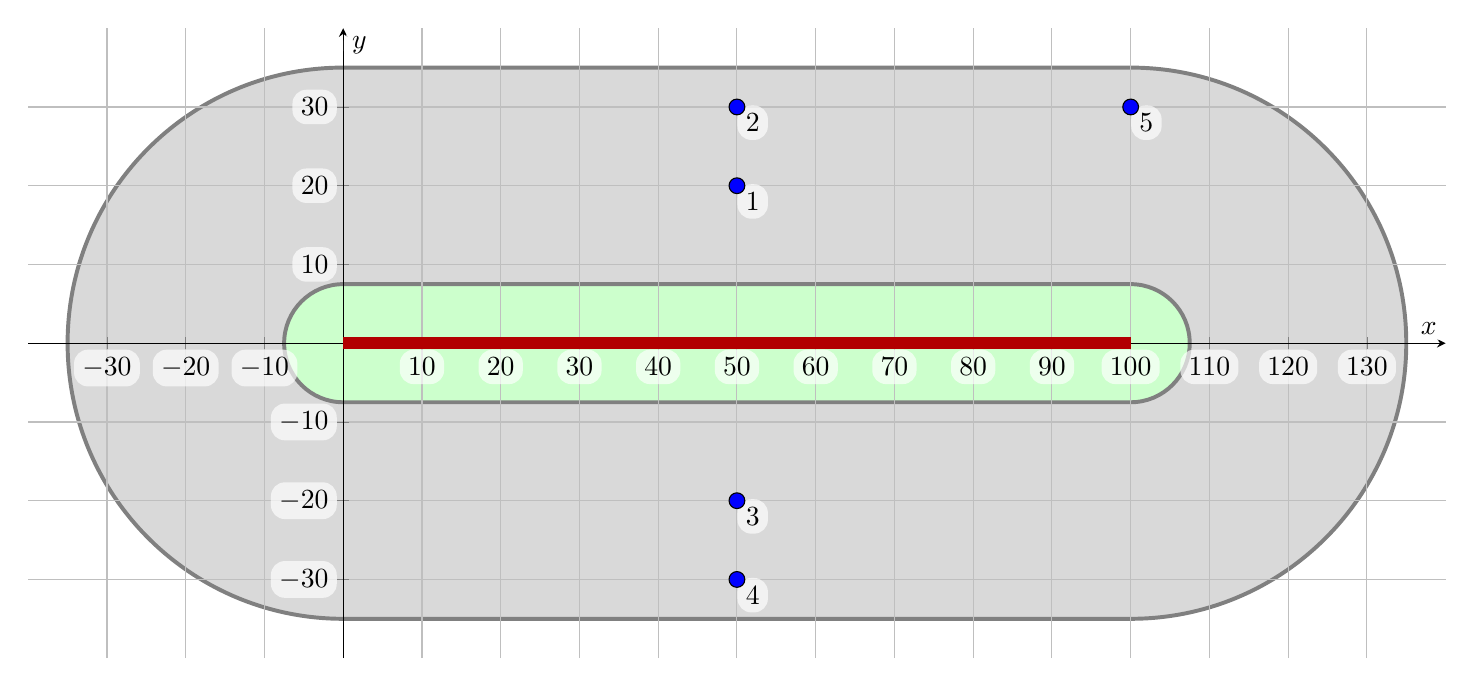
\begin{tikzpicture}[x=0.1cm,y=0.1cm]
		\begin{axis}[
			x=0.1cm,y=0.1cm,
			axis lines=middle,
			ymajorgrids=true,
			xmajorgrids=true,
			xmin=-40,
			xmax=140,
			ymin=-40,
			ymax=40,
			xtick={-30,-20,...,130},
			ytick={-30,-20,...,30},
			xlabel={$x$},
			ylabel={$y$},
			ticklabel style={fill=white,text opacity=1,fill opacity=0.66,inner sep=3pt,rounded corners=5pt},
			label style={fill=white,text opacity=1,fill opacity=0.66,inner sep=3pt,rounded corners=5pt},]
			\begin{scope}[on background layer]
				\draw[line width=0.05cm,black!50,fill=black!15,rounded corners=3.5cm] (-35, 35) rectangle (135, -35) {};
				\draw[line width=0.05cm,black!50,fill=green!20,rounded corners=0.75cm] (-7.5, 7.5) rectangle (107.5, -7.5) {};
			\end{scope}
			\newcounter{visitorID}
			\draw[color=red!70!black,line width=0.15cm] (0,0)--(100,0);
		\end{axis}
		\newcommand{\visitor}[2]{
			\stepcounter{visitorID}
			\node[fill=white,text opacity=1,fill opacity=0.66,inner sep=3pt,rounded corners=5pt] at (#1+42,#2+38) {$\arabic{visitorID}$};
			\draw [fill=blue] (#1+40,#2+40) circle (1);
		}
		%testdata:
		\visitor{50}{20}
		\visitor{50}{30}
		\visitor{50}{-20}
		\visitor{50}{-30}
		\visitor{100}{30}
	\end{tikzpicture}
\end{document} 
